\section{Homotopy Lie algebra and BRST}\label{sec:hla}
As we have seen in the \nameref{sec:ptfd}, asymptotic analysis of $\int e^{f/\hbar}$ leads to combinatorial formula via \emph{graphs} (Feynman diagram expansion) such as

propagator $P$: 
\( \begin{fmffile}{fde1}
    \begin{tabular}{c}
        \begin{fmfgraph*}(80,40)
                \fmfleft{i}
                \fmfright{o}
                \fmf{plain,label=$P$,l.side=left,tension=4}{i,o}
        \end{fmfgraph*}
        \end{tabular}
    \end{fmffile}
\),

vertex: 
\( \begin{fmffile}{fde2}
    \begin{tabular}{c}
        \begin{fmfgraph*}(100,50)
                \fmfleft{i1,i2}
                \fmfright{o}
                \fmf{plain,tension=4}{i1,v}
                \fmf{plain,tension=4}{i2,v}
                \fmf{plain,tension=4}{v,o}
                \fmfv{decor.shape=circle,decor.filled=full,decor.size=2thick}{v}
        \end{fmfgraph*}
        \end{tabular}
    \end{fmffile}
    , ~~~~~~~~ 
    \begin{fmffile}{fde3}
    \begin{tabular}{c}
        \begin{fmfgraph*}(100,50)
                \fmfleft{i1,i2}
                \fmfright{o1,o2}
                \fmf{plain,tension=4}{i1,v}
                \fmf{plain,tension=4}{i2,v}
                \fmf{plain,tension=4}{v,o1}
                \fmf{plain,tension=4}{v,o2}
                \fmfv{decor.shape=circle,decor.filled=full,decor.size=2thick}{v}
        \end{fmfgraph*}
        \end{tabular}
    \end{fmffile}
\).
    
Our next goal is to find its connection with constructions in homological algebra.

\subsection*{Differential graded Lie algebra (DGLA)}
    \begin{defn}
    A \textbf{graded Lie algebra} is a $\bZ$-graded vector space
    \bea \fg=\bigoplus_{k\in\bZ} \fg_k\eea
    with a bilinear map $\lsb -,-\rsb: \fg \otimes \fg \to \fg$
    satisfying the following conditions:
    \bi[(a)]
    \item (graded bracket) $\lsb \fg_\alpha, \fg_\beta\rsb \subset \fg_{\alpha+\beta}$,
    \item (graded skew-symmetry/anti-symmetry) $\lsb a,b\rsb=-(-1)^{\alpha\beta}\lsb b,a\rsb \ \text{for } a\in\fg_\alpha, b\in\fg_\beta$,
    \item (Jacobi identity) $\forall a\in\fg_\alpha$, $b\in\fg_\beta$, $c\in\fg_\gamma$,
    \bea \lsb a, \lsb b, c\rsb\rsb= \lsb \lsb a, b \rsb, c\rsb +(-1)^{\alpha\beta} \lsb b, \lsb a, c\rsb \rsb.\eea
    \ei
    \end{defn}
    
    \begin{defn}
    A \textbf{differential graded Lie algebra (DGLA)} is a graded Lie algebra $\fg$ with a differential $d$ of degree, $\on{deg}=1$ ($d: \fg_k \to\fg_{k+1}$), satisfying 
    \begin{itemize}
        \item $d^2=0$,
        \item $d\lsb a,b\rsb = \lsb da,b\rsb +(-1)^\alpha \lsb a, db\rsb$ for $a\in\fg_\alpha$, $b\in\fg_\beta$.
    \end{itemize}
    \end{defn}

\begin{eg}
An ordinary Lie algebra is a DGLA where
$\fg=\fg_0$ ($\fg$ is concentrated in $\on{deg}=0$) 
and $d=0$.
We see that DGLA is a natural generalization of Lie algebras.
\end{eg}

\begin{eg}
Let $X$ be a manifold and $\fg$ be a Lie algebra. Let $\lb \Omega^\blt(X),\ d\rb$ be the de Rham complex. Then 
$\lb \Omega^\blt(X) \otimes \fg,\ d,\ \lsb -,-\rsb_\fg \rb$
is a DGLA.
\begin{itemize}
    \item $\Omega^k \otimes \fg$ is a ($\on{deg}=k$)-component,
    \item $d: \Omega^k \otimes \fg \to \Omega^{k+1} \otimes \fg$ is a de Rham differential, where
    \bea d(\alpha\otimes h)= d\alpha\otimes h \quad \text{for } \alpha\in\Omega^\blt, h\in\fg,\eea
    \item the bracket is induced from the Lie bracket $\lsb -,-\rsb_\fg$ on $\fg$, where
    \bea \lsb \alpha_1\otimes h_1, \alpha_2\otimes h_2\rsb
    =(\alpha_1\wedge \alpha_2)\otimes \lsb h_1,h_2\rsb_\fg \quad \text{for any } \alpha_1,\alpha_2\in \Omega^\blt,\ h_1,h_2\in\fg.\eea
\end{itemize}
This example is related to Chern-Simons (CS) theory.
\end{eg}


\begin{eg}
Let $X$ be a complex manifold. Let $\lb \Omega^{0,\blt}(X),\pb\rb$ be the Dolbeault complex. Let $T^{1,0}_X$ denote the bundle of $(1,0)$-vector fields. Then $\lb \Omega^{0,\blt}(X, T^{1,0}_X),\pb, \lsb -,-\rsb\rb$ is a DGLA.
Explicitly, let $\lcb z^i\rcb$ be local holomorphic coordinates. 
An element of $\on{deg}=k$, $\alpha\in \Omega^{0,k}\lb X,T^{1,0}_X\rb$, can be written as 
\bea \alpha=\sum_{i,J} \alpha^i_{\ols J} d\zb^{\ols J}\otimes \p_{z^i}.\eea
Here $J=\lcb j_1,<\cdots< j_k\rcb$ is a multi-index and 
$d\zb^{\ols J}= d\zb^{j_1}\wedge\cdots\wedge d\zb^{j_k}$. Then the differential is 
\bea \pb \alpha = \sum_{i,J} \pb (\alpha^i_{\ols J}) \wedge d\zb^{\ols J} \otimes \p_{z^i}
= \sum_{i,J} \lb \pb_\ell \alpha^i_{\ols J}\rb d\zb^\ell \wedge d\zb^{\ols J} \otimes \p_{z^i}.\eea
Given two elements
\bea \alpha= \sum_{i,J} \alpha^i_{\ols J} d\zb^{\ols J} \otimes \p_{i}, \quad 
\beta= \sum_{i,M} \beta^i_{\ols M} d\zb^{\ols M} \otimes \p_{i},\eea
the bracket is given by
\bea \lsb \alpha,\beta\rsb= \sum_{i,j,J,M} \lb \alpha^j_{\ols J} \p_j \beta^i_{\ols M} -\beta^j_{\ols M}\p_j \alpha^i_{\ols J} \rb d\zb^{\ols J} \wedge d\zb^{\ols M} \otimes \p_i. 
\eea
On $\on{deg}=0$ components, this is just the usual Lie bracket on $(1,0)$-vector fields.
As we will study later, this example is related to the deformation of complex structures and also the so-called \emph{Kodaira-Spencer gravity} (this is the B-twisted topological closed string field theory, also known as the B-model).
\end{eg}

\subsection*{Chevalley-Eilenberg (CE) and BRST}
Let $\fg$ be a Lie algebra. Let $\fg^\vee$ be its linear dual. For simplicity, let us assume $\fg$ is finite dimensional.
Consider 
\bea C^\blt (\fg)= \bigoplus_k \asym^k \fg^\vee.\eea
This is a polynomial algebra in odd variables.
If we choose basis $\lcb e_\alpha\rcb $ of $\fg$, and dual basis $\lcb c^\alpha\rcb$ of $\fg^\vee$, then we can write
\bea C^\blt(\fg)= \bR\lsb c^\alpha\rsb,\eea
where $c^\alpha c^\beta= -c^\beta c^\alpha$.
Let $\lsb -,-\rsb: \asym^2 \fg \to \fg$ be the Lie bracket. Taking the dual, we find
$\lsb -,-\rsb^\vee: \fg^\vee \to \asym^2 \fg^\vee$.
This defines a \textbf{derivation} $d_{\on{CE}}$ on $C^\blt (\fg)$:
\bea d_{\on{CE}}: C^\blt(\fg) \to C^\blt(\fg)\eea
which is determined by the following properties:
\begin{itemize}
    \item on generators: $d_{\on{CE}}= \lsb -,-\rsb^\vee$ on $\fg^\vee$,
    \item $d_{\on{CE}}$ satisfies the graded Leibniz rule:
    \bea d_{\on{CE}}(a\wedge b)= \lb d_{\on{CE}} a\rb\wedge b +(-1)^k a\wedge d_{\on{CE}}(b) \quad \text{if } a\in C^k(g).\eea
\end{itemize}

\begin{prop}
$d_{\on{CE}}^2=0$.
\end{prop}
So $\lb C^\blt(\fg),d_{\on{CE}}\rb$ defines a complex, called the \textbf{Chevalley-Eilenberg (CE) complex}.
In fact, $d_{\on{CE}}^2=0$ is equivalent to Jacobi identity; this is a good exercise.
In terms of the above chosen basis, let
\bea \lsb e_\alpha, e_\beta \rsb= \sum_\gamma f^\gamma_{\alpha\beta} e_\gamma.\eea
Here $f^\gamma_{\alpha\beta}$ is the \emph{structure constant}. Then we have the explicit formula
\bea d_{\on{CE}}(c^\alpha)=\hf \sum_{\beta, \gamma} f^\alpha_{\beta \gamma} c^\beta c^\gamma.\eea
This is used in physics to describe the BRST formalism for gauge theory with the correspondences:
\bea c^\alpha &\lra \text{ghost field},\\
d_{\on{CE}} &\lra \text{BRST differential}.\eea
The above construction also generalizes to the case when we have a $\fg$-representation. Such $\fg$-representation is given by matter field in BRST formalism.

\subsection*{Linear algebra for graded vector spaces}
We will generalize the above construction to DGLA, and eventually to homotopic Lie algebras.

Let us first fix some conventions for graded spaces.
\begin{itemize}
    \item $W=\bigoplus_{n\in\bZ} W_n$ denotes a $\bZ$-graded vector space.
    
    \item $W[n]$ denotes the $\bZ$-graded vector space with a degree shift by $n$ where
    \bea W[n]_m \coloneqq W_{n+m}.\eea
    
\begin{figure}[!htpb]\centering
\tikzset{every picture/.style={line width=0.75pt}} %set default line width to 0.75pt        

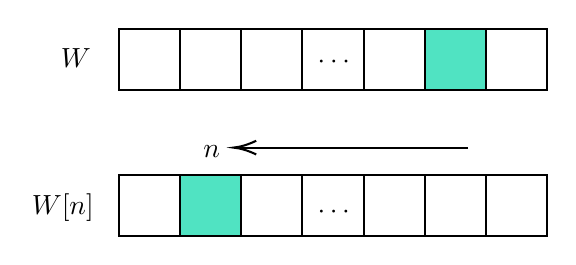
\begin{tikzpicture}[x=0.75pt,y=0.75pt,yscale=-1,xscale=1]
%uncomment if require: \path (0,300); %set diagram left start at 0, and has height of 300

%Shape: Square [id:dp0812615772659322] 
\draw   (130.67,41.72) -- (160.17,41.72) -- (160.17,71.22) -- (130.67,71.22) -- cycle ;
%Shape: Square [id:dp9156482978414704] 
\draw   (160.17,41.72) -- (189.67,41.72) -- (189.67,71.22) -- (160.17,71.22) -- cycle ;
%Shape: Square [id:dp8589697057894725] 
\draw   (189.67,41.72) -- (219.17,41.72) -- (219.17,71.22) -- (189.67,71.22) -- cycle ;
%Shape: Square [id:dp5527310059356019] 
\draw   (219.17,41.72) -- (248.67,41.72) -- (248.67,71.22) -- (219.17,71.22) -- cycle ;
%Shape: Square [id:dp3340966716018581] 
\draw   (248.67,41.72) -- (278.17,41.72) -- (278.17,71.22) -- (248.67,71.22) -- cycle ;
%Shape: Square [id:dp1473977553017456] 
\draw  [fill={rgb, 255:red, 80; green, 227; blue, 194 }  ,fill opacity=1 ] (278.17,41.72) -- (307.67,41.72) -- (307.67,71.22) -- (278.17,71.22) -- cycle ;
%Shape: Square [id:dp06348149501159495] 
\draw   (307.67,41.72) -- (337.17,41.72) -- (337.17,71.22) -- (307.67,71.22) -- cycle ;
%Shape: Square [id:dp4355149690645379] 
\draw   (130.67,112.22) -- (160.17,112.22) -- (160.17,141.72) -- (130.67,141.72) -- cycle ;
%Shape: Square [id:dp24955859820800752] 
\draw  [fill={rgb, 255:red, 80; green, 227; blue, 194 }  ,fill opacity=1 ] (160.17,112.22) -- (189.67,112.22) -- (189.67,141.72) -- (160.17,141.72) -- cycle ;
%Shape: Square [id:dp7712136013152768] 
\draw   (189.67,112.22) -- (219.17,112.22) -- (219.17,141.72) -- (189.67,141.72) -- cycle ;
%Shape: Square [id:dp13940177538276122] 
\draw   (219.17,112.22) -- (248.67,112.22) -- (248.67,141.72) -- (219.17,141.72) -- cycle ;
%Shape: Square [id:dp4166608510635037] 
\draw   (248.67,112.22) -- (278.17,112.22) -- (278.17,141.72) -- (248.67,141.72) -- cycle ;
%Shape: Square [id:dp6958291315519955] 
\draw   (278.17,112.22) -- (307.67,112.22) -- (307.67,141.72) -- (278.17,141.72) -- cycle ;
%Shape: Square [id:dp3744108591086348] 
\draw   (307.67,112.22) -- (337.17,112.22) -- (337.17,141.72) -- (307.67,141.72) -- cycle ;
%Straight Lines [id:da8996678375365978] 
\draw    (299,99) -- (188,99) ;
\draw [shift={(186,99)}, rotate = 360] [color={rgb, 255:red, 0; green, 0; blue, 0 }  ][line width=0.75]    (10.93,-3.29) .. controls (6.95,-1.4) and (3.31,-0.3) .. (0,0) .. controls (3.31,0.3) and (6.95,1.4) .. (10.93,3.29)   ;

% Text Node
\draw (101.33,49.62) node [anchor=north west][inner sep=0.75pt]    {$W$};
% Text Node
\draw (87.33,119.62) node [anchor=north west][inner sep=0.75pt]    {$W[n]$};
% Text Node
\draw (170,96.5) node [anchor=north west][inner sep=0.75pt]    {$n$};
% Text Node
\draw (225,53.5) node [anchor=north west][inner sep=0.75pt]  [rotate=-359.39]  {$\cdots $};
% Text Node
\draw (225,125.5) node [anchor=north west][inner sep=0.75pt]    {$\cdots $};

\end{tikzpicture}
\end{figure}
    
    \item $W^\vee$ denotes the linear dual with 
    \bea W^\vee_m=\on{Hom}(W_{-m},\mathbf{k}) \quad \text{for base field } \mathbf{k}. \eea
    
    \item Given two $\bZ$-graded vector spaces $V$, $W$, with base field being implicit,
    \bea \lb V\otimes W\rb_n &=\bigoplus_{i+j=n} \lb V_i\otimes W_j\rb,\\
    \on{Hom}(V,W)_n
    &= \bigoplus_i \on{Hom}(V_i, W_{i+n}).\eea
    
    \item $\sym^m(V)$ denotes a $m$-th graded symmetric tensor, which is $V^{\otimes m}/\sim$ where $a\otimes b\sim +(-1)^{|a||b|}b\otimes a$ (here $|a|$ is the parity of $a$).
    
    \item $\asym^m(V)$ denotes a $m$-th graded skew-symmetric tensor, which is $V^{\otimes m}/\sim$ where $a\otimes b\sim -(-1)^{|a||b|} b\otimes a$.

    \item We will write 
    $\sym(V)=\bigoplus_{m\geq 0} \sym^m(V)$ as the (graded) polynomial ring generated by $V$ and  $\widehat{\sym}(V)=\prod_{m\geq 0} \sym^m(V)$ as the (graded) formal power series ring generated by $V$.
\end{itemize}

\begin{prop}We have $\asym^k(V[1])\simeq \sym^k(V)[k]$.
\end{prop}
\begin{proof}
A very helpful exercise for the reader.
\end{proof}


\subsection*{CE complex for DGLA}
Let $(g,d,[-,-])$ be a DGLA. Let
\bea C^\blt(\fg)\coloneqq \sym^\blt(\fg^\vee[-1]).\eea
Since $\fg^\vee[-1]= \lb \fg[1]\rb^\vee$, $\sym^\blt \lb\fg^\vee[-1]\rb = \sym^\blt\lb \fg[1]\rb^\vee$, we can think of $C^\blt(\fg)$ as a (polynomial) function on $\fg[1]$. 
When $\fg$ is a Lie algebra,
\bea C^k(\fg)= \sym^k\lb \fg^\vee[-1]\rb\simeq \asym^k \fg^\vee[-k].\eea
This is $\asym^k \fg^\vee$ sitting at degree $k$. We get the usual CE.

Let 
\bea d_\fg: \fg^\vee[-1]\to \fg^\vee[-1]\eea
be the dual of $d:\fg \to \fg$ and \bea d_{[-,-]}:\fg^\vee[-1]\to \sym^2(\fg^\vee[-1])\simeq \asym^2 \fg^\vee[-2]\eea
be the dual of the bracket $[-,-]: \asym^2 \fg \to\fg$. Note that both $d_\fg$ and $d_{[-,-]}$ have $\on{deg}=1$ (check!).

Since $C^\blt(\fg)$ is freely generated by $\fg^\vee[-1]$, we can extend $d_\fg$ and $d_{[-,-]}$ to $C^\blt(\fg)$ by requiring them to
\begin{itemize}
    \item act on the generator $\fg^\vee[-1]$, as defined above,
    \item satisfy the graded Leibniz rule.
\end{itemize}

Define the \textbf{CE differential}
\bea d_{\on{CE}} \coloneqq d_\fg +d_{[-,-]}.\eea

\begin{clm}
$d_{\on{CE}}^2=0$.
\end{clm}
\begin{sproof}
We illustrate why this is true and leave the details to readers. In fact, if we represent

\bea
d_{\on{CE}}: \begin{fmffile}{dce1a}
    \begin{tabular}{c}
        \begin{fmfgraph*}(100,60)
                \fmfleft{i}
                \fmfright{o}
                \fmf{fermion,label=$d$,l.side=left,tension=4}{i,o}
        \end{fmfgraph*}
        \end{tabular}
    \end{fmffile}
    ~~~ + ~~~
    \begin{fmffile}{dce1b}
    \begin{tabular}{c}
        \begin{fmfgraph*}(100,60)
                \fmfleft{i1,i2}
                \fmfright{o}
                \fmf{fermion,tension=4}{i1,v}
                \fmf{fermion,tension=4}{i2,v}
                \fmf{fermion,tension=4}{v,o}
                \fmfv{label=$[-,,-]$,l.angle=45,decor.shape=circle,decor.filled=full,decor.size=2thick}{v}
        \end{fmfgraph*}
        \end{tabular}
    \end{fmffile},
\eea
then
\bea
d_{\on{CE}}^2: &
\begin{fmffile}{dce2a}
    \begin{tabular}{c}
        \begin{fmfgraph*}(100,50)
                \fmfleft{i}
                \fmfright{o}
                \fmf{fermion,label=$d^2$,l.side=left,tension=4}{i,o}
        \end{fmfgraph*}
        \end{tabular}
    \end{fmffile}
    \\ ~~~ & + ~~~
    \begin{fmffile}{dce2b}
    \begin{tabular}{c}
        \begin{fmfgraph*}(100,60)
                \fmfleft{i1,i2}
                \fmfright{o}
                \fmf{fermion,label=$d$,l.side=left,tension=4}{i2,v}
                \fmf{fermion,tension=4}{i1,v}
                \fmf{fermion,tension=5}{v,o}
                \fmfv{decor.shape=circle,decor.filled=full,decor.size=2thick}{v}
        \end{fmfgraph*}
        \end{tabular}
    \end{fmffile}
    ~~~ + ~~~
    \begin{fmffile}{dce2c}
    \begin{tabular}{c}
        \begin{fmfgraph*}(100,60)
                \fmfleft{i1,i2}
                \fmfright{o}
                \fmf{fermion,tension=4}{i2,v}
                \fmf{fermion,label=$d$,l.side=right,tension=4}{i1,v}
                \fmf{fermion,tension=5}{v,o}
                \fmfv{decor.shape=circle,decor.filled=full,decor.size=2thick}{v}
        \end{fmfgraph*}
        \end{tabular}
    \end{fmffile}
    ~~~ + ~~~
    \begin{fmffile}{dce2d}
    \begin{tabular}{c}
        \begin{fmfgraph*}(100,60)
                \fmfleft{i1,i2}
                \fmfright{o}
                \fmf{fermion,tension=4}{i1,v}
                \fmf{fermion,tension=4}{i2,v}
                \fmf{fermion,label=$d$,l.side=left,tension=5}{v,o}
                \fmfv{decor.shape=circle,decor.filled=full,decor.size=2thick}{v}
        \end{fmfgraph*}
        \end{tabular}
    \end{fmffile}
    \\ ~~~ & + ~~~
    \sum_{\text{permutations}} \lb
    \begin{fmffile}{dce2e}
    \begin{tabular}{c}
        \begin{fmfgraph*}(120,80)
                \fmfleft{i1,i2,i3}
                \fmfright{o}
                \fmf{fermion,tension=1}{i1,v2}
                \fmf{fermion,tension=1}{i2,v1}
                \fmf{fermion,tension=1}{i3,v1}
                \fmf{fermion,tension=2}{v1,v2}
                \fmf{fermion,tension=2}{v2,o}
                \fmfv{label=$[-,,-]$,l.angle=65,decor.shape=circle,decor.filled=full,decor.size=2thick}{v1}
                \fmfv{label=$[-,,-]$,l.angle=65,decor.shape=circle,decor.filled=full,decor.size=2thick}{v2}
        \end{fmfgraph*}
        \end{tabular}
    \end{fmffile}\rb.
\eea

We can ``see'' that 
$d_{\on{CE}}^2=0$ is equivalent to the defining properties of DGLA:
\begin{itemize}
    \item $d^2=0$,
    \item Leibniz rule: $d\lsb-,-\rsb=\lsb d(-),-\rsb\pm \lsb -,d(-)\rsb$,
    \item Jacobi identity.
\end{itemize}
$\lb C^\blt(\fg),d_{\on{CE}}\rb$ is called the \textbf{CE complex}.
\end{sproof}


\subsection*{Homotopy Lie algebra ($L_\infty$-algebra)}
Given a graded vector space $V$, we consider a (graded) derivation 
on $\sym(V)$:
\bea \delta: \sym(V) \to \sym(V),\eea
which satisfies the graded Leibniz rule
\bea \delta(a\otimes b)=(\delta a)\otimes b \pm a\otimes \delta b.\eea 
Such $\delta$ is completely determined by how $\delta$ acts on the generator
\bea \delta: V\to \sym(V).\eea

We can decompose
\bea \delta=\delta_0+\delta_1+\delta_2+\cdots,\eea
where $\delta_k:V\to \sym^k(V).$
For DGLA, we have $d_{\on{CE}}$ acting on $C^\blt(\fg)=\sym(\fg^\vee\lsb -1\rsb)$, where \bea d_{\on{CE}}=d_\fg+d_{[-,-]} =\delta_1+\delta_2.\eea
This is a derivation where only $\delta_1$, $\delta_2$ are nontrivial. It is natural to generalize this operator by encoding all possible components $\delta_k$. This leads to the \emph{$L_\infty$-algebra}.


\begin{defn}
An \textbf{$L_\infty$-algebra} is a $\bZ$-graded vector space $\fg$ with a collection of multilinear maps
\bea \ell_n: \asym^n \fg \to \fg, \quad \on{deg}(\ell_n)=2-n \quad (n\geq 1)\eea
satisfying the following $L_\infty$-relation
\bea \sum_{k=1}^n \pm \ell_{n-k+1}\lb \ell_k\lb \cdots\rb, \cdots\rb=0 \quad \forall n.\eea
\end{defn}
 
The complicated $L_\infty$-relation can be understood as follows. Let
\bea \delta_n: \fg^\vee\lsb-1\rsb \to \sym^n\lb \fg^\vee\lsb-1\rsb\rb\simeq \asym^n \fg^\vee \lsb-n\rsb\eea
denotes the dual of $\ell_n:\asym^n \fg\to\fg$. Note that
\bea \on{deg}(\ell_n)=2-n \ \LRA\ \on{deg}(\delta_n)=1.\eea
Let $\delta=\sum_{n\geq 1}\delta_n= \delta_1+\delta_2+\cdots$ defines a derivation on $C^\blt(\fg)=\widehat{\sym}\lb \fg^\vee\lsb -1\rsb\rb$ via the graded Leibniz rule. (Here we use the (graded) formal power series ring $\widehat{\sym}\lb \fg^\vee\lsb -1\rsb\rb$ so that $\delta$ is defined.) Then
\bea L_\infty \text{-relations for } \lcb \ell_n\rcb_{n\geq 1}\ \LRA\ \delta^2=0.\eea
$\lb C^\blt(\fg),\delta\rb$ is the CE complex for $\fg$.

If we represent each $\delta_n$ as a graph
\bea
n\lcb ~~~
    \begin{fmffile}{dce3}
    \begin{tabular}{c}
        \begin{fmfgraph*}(150,120)
                \fmfleft{i1,i2,i3,i4,i5,i6,i7,i8,i9,i10}
                \fmfright{o}
                \fmf{fermion,tension=1}{i10,v}
                \fmf{phantom,tension=1}{i9,v}
                \fmf{fermion,tension=1}{i8,v}
                \fmf{phantom,tension=1}{i7,v}
                \fmf{phantom,tension=1}{i6,v}
                \fmf{phantom,tension=1}{i5,v}
                \fmf{phantom,label=$\cdot$,l.side=left,tension=1}{i4,v}
                \fmf{phantom,label=$\cdot$,l.side=left,tension=1}{i3,v}
                \fmf{phantom,label=$\cdot$,l.side=left,tension=1}{i2,v}
                \fmf{fermion,tension=1}{i1,v}
                \fmf{fermion,tension=5}{v,o}
                \fmfv{label=$\ell_n$,label.angle=45,decor.shape=circle,decor.filled=full,decor.size=2thick}{v}
        \end{fmfgraph*}
        \end{tabular}
    \end{fmffile}
    \right.,
\eea
then $\delta^2=0$ can be pictured as 
\bea \sum_{\text{permutations}}\lb
    \begin{fmffile}{dce4}
        \begin{tabular}{c}
        \begin{fmfgraph*}(200,150)
                \fmfleft{h1,h2,h3,h4,h5,h6,h7,h8,h9,h10,i1,i2,i3,i4,i5,i6,i7,i8,i9,i10,i11,i12}
                \fmfright{o}
                \fmf{fermion,tension=1}{i12,v}
                \fmf{phantom,tension=1}{i11,v}
                \fmf{phantom,tension=1}{i10,v}
                \fmf{fermion,tension=1}{i9,v}
                \fmf{phantom,tension=1}{i8,v}
                \fmf{phantom,tension=1}{i7,v}
                \fmf{phantom,tension=1}{i6,v}
                \fmf{phantom,tension=1}{i5,v}
                \fmf{phantom,label=$\cdot$,l.side=left,tension=1}{i4,v}
                \fmf{phantom,label=$\cdot$,l.side=left,tension=1}{i3,v}
                \fmf{phantom,label=$\cdot$,l.side=left,tension=1}{i2,v}
                \fmf{fermion,tension=1}{i1,v}
                
                \fmf{fermion,tension=10}{h10,w}
                \fmf{phantom,tension=10}{h9,w}
                \fmf{phantom,tension=10}{h8,w}
                \fmf{phantom,tension=10}{h7,w}
                \fmf{phantom,tension=10}{h6,w}
                \fmf{phantom,tension=10}{h5,w}
                \fmf{phantom,label=$\cdot$,l.side=left,tension=10}{h4,w}
                \fmf{phantom,label=$\cdot$,l.side=left,tension=10}{h3,w}
                \fmf{phantom,label=$\cdot$,l.side=left,tension=10}{h2,w}
                \fmf{fermion,tension=10}{h1,w}
                
                \fmf{fermion,tension=10}{v,w}
                \fmf{fermion,tension=150}{w,o}
                \fmfv{label=$\ell_n$,label.angle=60,decor.shape=circle,decor.filled=full,decor.size=2thick}{v}
                \fmfv{label=$\ell_n$,label.angle=60,decor.shape=circle,decor.filled=full,decor.size=2thick}{w}
        \end{fmfgraph*}
        \end{tabular}
    \end{fmffile}
    \rb=0.
\eea

As we will see, this has a natural interpretation via Feynman diagram technique.

\noindent \textsc{References}:
\cite{Lada:2021vvm} and its references for a nice review on $L_\infty$-algebra and its relation in QFT,
\cite{Li:2018rnc} for a self-contained review on $L_\infty$-algebra which we are following in this lecture.
